% Checklist and Procedures
\chapter{Checklists and Procedures}
\section{PECVD}
\subsection{WLO1}
\subsubsection{Checklist}
\begin{enumerate}
\item Turbo Pumps: 37 kRPM, 17 - 19 \superscript{o}C.
\item Ion gauges (PL2 - PL4): $ \leq $ 10\superscript{-6} Torr.
\item LL(Load Lock) gate valve pressure: $ \leq $ 20 $\times$ 10\superscript{-2} Torr, or 20 mTorr range.
\item Temperature matching should take 1 -- 1.5 hours.
\item Process Parameter Limits.
  \begin{enumerate}
  \item Max substrate heater temperature: 500 \superscript{o}C.
  \item Turbo Pumps: Max total gas flow should be $\leq$ 250 sccm.
  \item Turbo Pumps: Max temperature, 60 \superscript{o}C.
  \item Max chamber process pressure: 2 Torr (or 2000 mTorr)
  \item MFCs
    \begin{itemize}
    \item SiH\subscript{4}, B\subscript{2}H\subscript{6}, %
      PH\subscript{3} = 50 sccm
    \item NH\subscript{3} = 500 sccm (recommended: 100 sccm)
    \item H\subscript{2} = 500 sccm (recommended: 250 sccm)
    \end{itemize}
  \end{enumerate}
\item Hardware Configuration
  \begin{itemize}
  \item PL1 -- Load Lock
  \item PL2 -- Undoped a-Si:H or nc-Si:H
  \item PL3 -- n+ a-Si:H/nc-Si:H
  \item PL5 -- Si Sputtering
  \item PL7 -- Excimer laser annealing
  \item ITZ -- Robotic arm transport 
  \end{itemize}
\end{enumerate}

\subsubsection{Procedures}
This section was written assuming a-Si:H deposition in PL2 chamber. Make sure main gas valves are opened in gas line controller next to process room prior to deposition. MFC(Mass Flow Controller) valves are usually turned on for WLO1 unlike Reel-to-Reel machine. The gas cylinder pressure, check them in the gas line controller room, should be over 100 psi.
\begin{enumerate}
  \item Vent the Load Lock and prepare substrate holder with samples.
  \item Put holder back to the Load Lock and close door.\footnote{Keep a 5 mm gap}
  \item 'Rough' until the Load Lock pressure become 20 mTorr. \\
    Don't forget to close 'Rough' valve if the pressure is low enough. Too low pressure might reverse the lubricant oil from rotary pump and contaminate the samples.
  \item Check ITZ pressure ($<$ 10\superscript{-6}) using Ion Gauge (IG).
  \item Open Gate Valve 1 (GV1).
  \item From robotic arm panel, select Chamber $\rightarrow$ Load Lack and hit 'Get' button. Robot arm will take out the wafer holder from Load Lock and stay at ITZ.
  \item Close GV1 and open GV2. Check whether GV2 is opened.
  \item Again, from the robotic arm panel, select Chamber $\rightarrow$ PL2 and hit 'Put' button to place the substrate holder into the PL2. Confirm the robot arm action is finished prior to close GV2.
  \item Close GV2 and setup the process parameters. 
  \item Wait until substrate temperature reaches desired temperature. It takes about 1 hour.
  \item Press the MFC, Gas Valve, and Main Valve buttons connected to PL2.
  \item Hit 'Pr' (Pressure) button to setup chamber pressure and wait until desired pressure achieved.
  \item Hit 'Tm' (Timer) button to ignite plasma. To confirm the plasma visually, look through the PL2 chamber via look glass. If the plasma is not ignited, turn off the timer and increase RF power a bit and try to re-ignite the plasma. 
  \item Always check the plasma, gas flow, pressure during deposition process.
  \item Once the plasma confirmed, wait until timer value dissipates to zero. The RF will automatically run off once the timer finishes. 
  \item Hit 'Op' for Throttle valve. Turn off very gas valves, MFCs connected to PL2. Wait until PL2 base pressure drop under 10\superscript{-6} Torr level.
  \item Open GV2, hit 'Get' at the robotic arm control panel after selecting PL2 chamber to take out the substrate holder from PL2. 
  \item Close GV2 and open GV1. 'Put' the substrate holder in the robotic arm control panel.
  \item Once the robotic arm is secured in ITZ, close GV1 and wait for 1 -- 1.5 hours to cool down the substrate holder.
  \item Vent the Load Lock and retrieve your samples. Don't forget to return Load Lock pressure at 2 $\times$ 10\superscript{-2} Torr, or 20 mTorr using 'Rough'.
\end{enumerate}

\subsection{Robot Arm Manipulation}
Due to the malfunction problem of the robot arm, we decided to operate the robot arm manually when moving the wafer tray into the load lack(LL). The procedure below assumes the wafer tray is located in the ITZ, mounted on the robot arm.
	\begin{enumerate}
		\item Open the gate valve of LL to see the robot arm operation.
		\item Operate the robot arm normally: LL, then Put.
		\item Stop the robot arm when it starts move towards LL by pressing `F1' on the keypad.
		\item Hit `LP1' (Learn Position 1) on the keypad then press `ENTER'.
		\item While holding `CTRL', press `$($B' 6 times.
		\item Hold `$>$E' until the substrate tray is 1 cm away from the stopper.
		\item Hold `-F' to lower the substrate tray to settle down in the LL.
		\item Hold `$<$D' until the robot arm is out of the LL chamber.
		\item Hit `RS1' then `ENTER' to reset the robot arm.
		\item Wait until a second beep then close the LL gate valve.
	\end{enumerate}

\pagebreak
\subsection{Plasmatherm}
\subsubsection{Checklist}

\begin{figure}[htp]
\centering
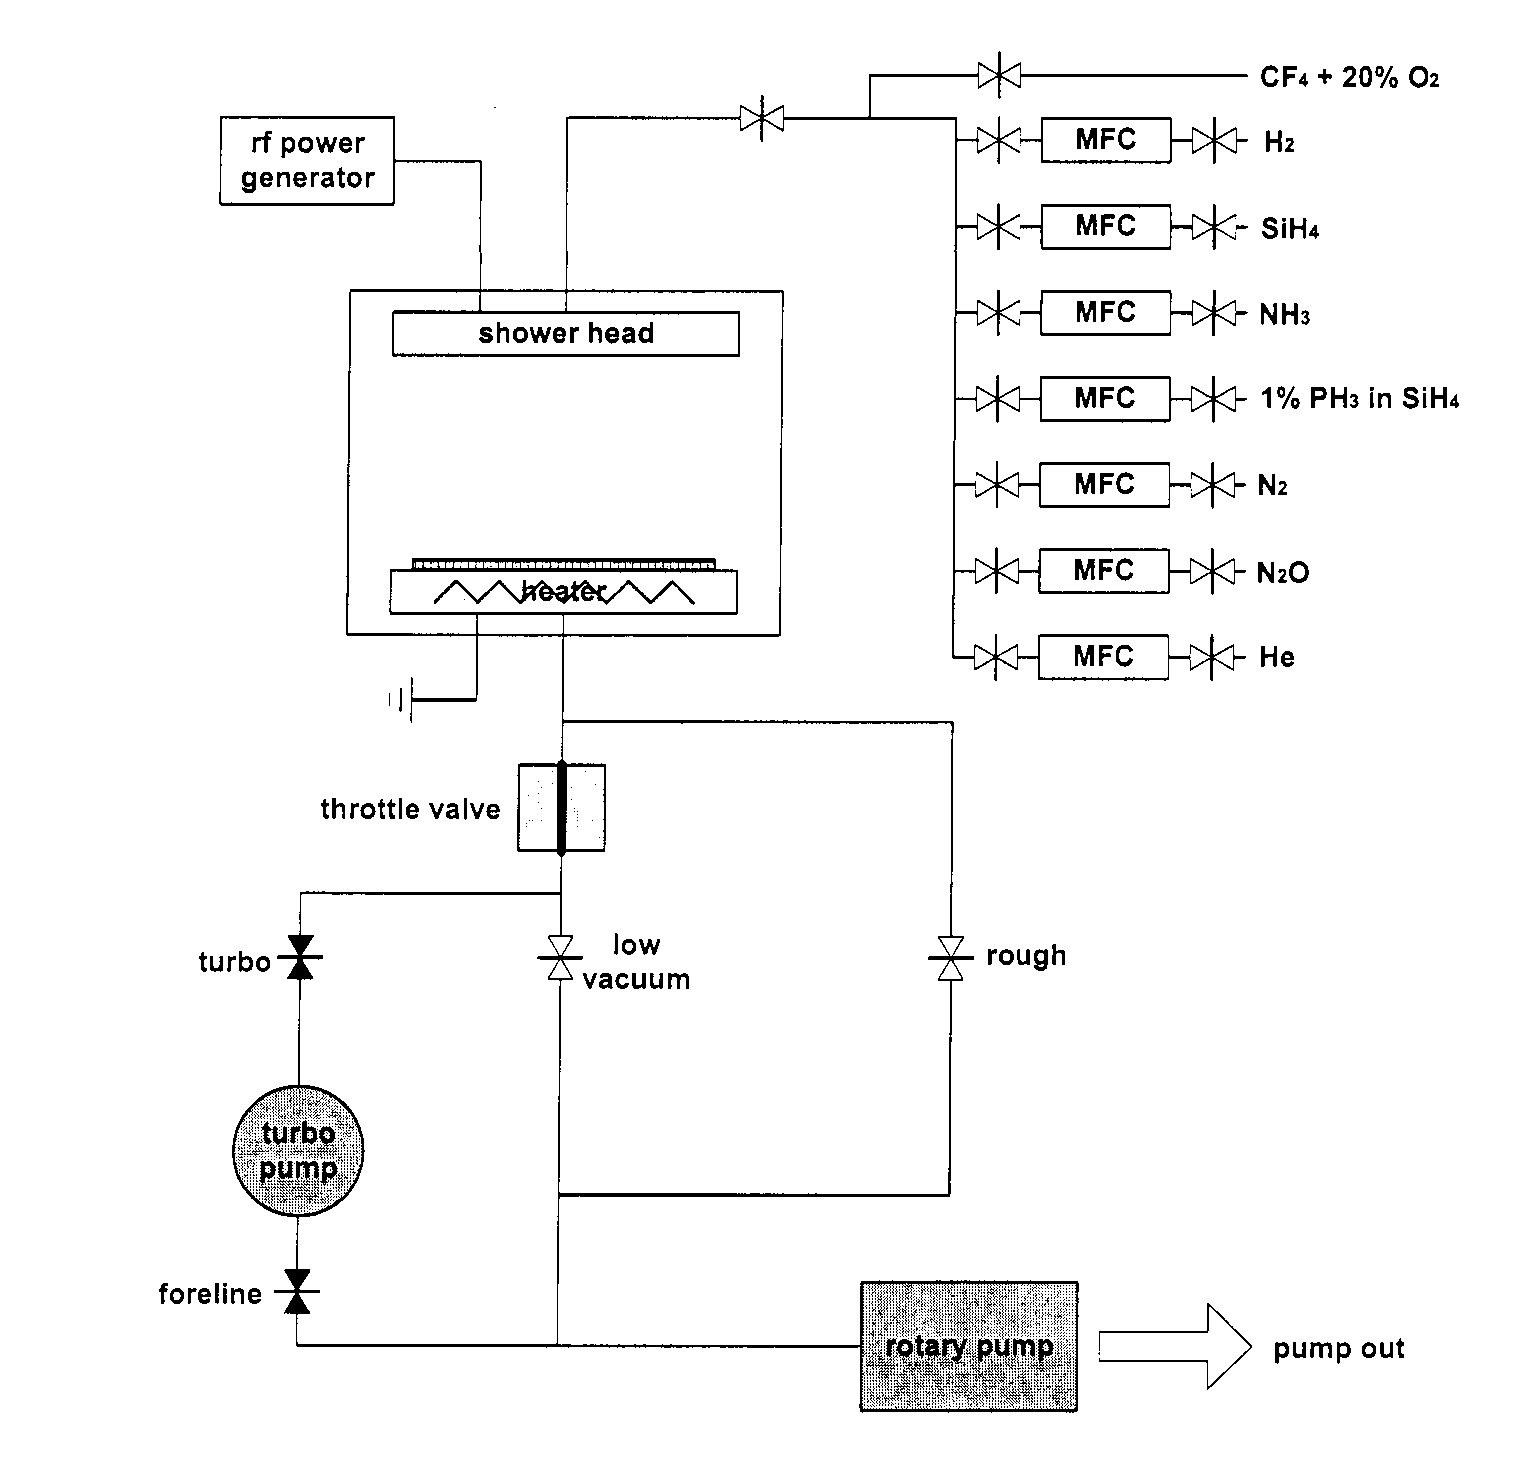
\includegraphics[width=.8\textwidth]{./img/plasmatherm.png}
\captionof{figure}{Schematic of Plasmatherm. Adopted from CzangHo Lee's thesis.}
\label{fig:Plasmatherm}
\end{figure}

\begin{enumerate}
\item Standby Temperature: 130 \superscript{o}C
\item Standby Pressure (Chamber): less than 1 $\times$ 10\superscript{-5} Torr.
\item The chamber must be cleaned prior to actual usage. (Use hi\_lo\_pr.prc)
\item In the back room (Gas control room), check whether rotary pumps working.
\item Prepare some glass plates and dummy wafers to prevent flying sample wafer accident.
\item Cleaning process is a mandatory one since the system has only a single process chamber.
\item Schematic can be found at Fig. \ref{fig:Plasmatherm}.
\end{enumerate}

\subsubsection{Procedure}
\begin{enumerate}
\item First, close main valve gate to prevent any possible damage to pumps. \\
Utilities $\rightarrow$ Close Gate
\item After confirming the gate is fully closed, Vent the chamber. \\
Utilities $\rightarrow$ Vent
\item Open the chamber after hearing 'tsk' sound from pumping mechanism. It indicates the chamber can be opened. (The panel shows 'cyan' colored process chamber when it is ready to open)
\item Place your wafers carefully. Try to place them in the middle of chamber.
\item Close chamber and start pumping with 'Low Vac' pump. Pump it until the chamber panel shows 'white' color. 
\item From this point, use 'Turbo' pump to achieve Hivac condition. It will take at least from the point that we turn on the 'Turbo' pump.
\item Wait until the chamber pressure reaches below 10\superscript{-5} Torr. Confirm this using ION gauge. Turn off ION gauge as soon as confirming pressure to preserve its lifetime.
\item Revise your process recipe ('.prc' file) and Load it. \\
Process $\rightarrow$ Edit/Process $\rightarrow$ Load
\item Press 'Ready' button at the bottom side of process control program. It will automatically setup the substrate temperature as your desired temperature.
\item Once the substrate temperature reaches recipe value, 'Run' the process. The process usually ends with Helium flush and cooling down procedure so that we can open the chamber right after process ends.
\item Follow previous procedures to open the chamber and unload samples.
\item Follow previous procedures to vacuum the chamber and run the cleaning process and leave. \\
Cleaning process can be found at 'C:$\backslash$sysmon$\backslash$cleaning'. Use 'hi\_lo\_pr.prc'.
\end{enumerate}

% PECVD section ends


% Sputtering section begins
\section{Sputtering}
\subsection{WLOS}
\subsubsection{Checklist}
\begin{enumerate}
\item Turbo Pumps: 37 kRPM, 17 -- 18 \superscript{o}C
\item MPZ Pressure (Vacuum): $<$ 5 $\times$ 10\superscript{-6} Torr
\item Load Lock Pressure: $\leq$ 2 $\times$ 10\superscript{-2} Torr
\item Bias Setup
  \begin{enumerate}
  \item Aluminum\footnote{Requires manual adjustment on target}/%
    Chromium\footnote{ITO is actually Chromium}: DC
  \item Molybdenum: RF (AC)		
  \end{enumerate}
\item Preferred substrate moving profile: 'wlosfull.SFS'
\end{enumerate}

% Subsection for firmware setup
\subsubsection{Substrate movement profile setup}
\begin{enumerate}
\item At the control terminal desktop,  \\ %
  Start $\Rightarrow$ Program $\Rightarrow$ % 
  Applied Motion Products $\Rightarrow$ %
  Si Programming
\item At the Si Programming window, \\ %
  Open $\Rightarrow$ Go to 'C:$\backslash$SiProg' $\Rightarrow$ Select 'wlosfull.SFS'%
  $\Rightarrow$ Open.
\item Now, 'wlosfull' program is loaded on SiProgrammer. Time to write the program to internal memory of the machine. \\
  Click 'Download' $\Rightarrow$ Execute\footnote{in the new pop-up window} %
  $\Rightarrow$ Run $\Rightarrow$	Close the New control panel and SiProg
\item Reset Indexer Switch at the left side of the machine. 
\end{enumerate}

% Subsection for actual process
\subsubsection{Deposition and Retrieving substrate holder}
\begin{enumerate}
\item Vent Load Lock. \\
  Don't forget to loosen the Load Lock lockers. Also, prepare the substrate holder.
\item Load substrate holder. \\
  Make sure substrate holder teeth match with one of saw-wheel inside. %
  The machine cannot transport the substrate holder to load position by itself. % 
\item Press 'Move $\rightarrow$ Load' button after placing substrate holder. %
  Then, close the Load Lock and tighten lockers.
\item 'Vent' the Load Lock down to 2 $\times$ 10\superscript{-2} Torr
\item When the Load Lock pressure is low enough. Open Gate Valve (GV), %
  then press 'Load $\rightarrow$ Start'  to deliver the substrate holder.
\item Close GV and wait until MPZ pressure become 5 $\times$ 10\superscript{-5} Torr.
  Setup the process parameters during this process.
\item Open Ar supply. Wait for pressure stabilized. 
\item Apply RF/DC power. A slightly higher power is recommended to ignite plasma. Also, wait for 2 -- 5 minutes for target surface cleaning.
\item Hit 'Timer' button to begin substrate oscillation. The oscillation will finish at the start location once timer runs out. Therefore, wait until the substrate holder stops at start position.
\item Open GV and press 'Start $\rightarrow$ Unload' to deliver the substrate holder to Load Lock.
\item Close GV and vent Load Lock to obtain metal deposited film. \\
  Don't forget to return the Load Lock pressure to standby value: 2 $\times$ 10\superscript{-2} Torr.
\end{enumerate}

% Edwards
\subsection{Edwards Sputter}
\subsubsection{Checklist}
\begin{enumerate}
\item Cryo-Pump temperature: $<$ 20 \superscript{o}K.
\item Chamber standby pressure: 10\superscript{-6} Torr. (Hi-Vac)
\item Manifold pressure: 10\superscript{-2} Torr range.
\item Target setting. (Al, Cr, Mo)
\item RF panel.
\item RF ground electrode.
\item Pumping Operation Overview.
  \begin{enumerate}
  \item Rotary Pump (Low-Vac): 760 Torr (Air pressure) $\rightarrow$ 10\superscript{-3} Torr. (It should be turned off when low pressure since the pressure difference back-flows the Rotary Pump oil.
  \item Cryo-Pump (Hi-Vac): 10\superscript{-3} Torr (Sometimes the Rotary Pump cannot run less than 5\superscript{-2} range. In this case, just continue to Cryo-Pump phase) $\rightarrow$ 10\superscript{-6} Torr. It \emph{MUST NOT} be exposed to air pressure due to the delicate mechanism of the pump itself. It takes at least a day to regenerate the Cryo, in the worst case, at least a month to replace the Cryo pump.
  \item All pumps \emph{MUST BE BLOCKED} before opening the Air Admit.
  \end{enumerate}
\item Manifold Control Valve.
  \begin{enumerate}
  \item Roughing: The pump is opened to chamber.
  \item Backing: The pump is isolated from chamber.
  \item Upper Half Circle/Lifted State: Cryo-Pump operation.
  \item Lower Side/Pushed State: Rotary Pump operation.
  \item 180\superscript{o} location implies both pumps are isolated from the sputtering chamber.
  \end{enumerate}
\item Always be gentle since the machine is older than a 30 years old nerd.
\end{enumerate}

\subsubsection{Wafer Loading/Vacuuming}
\label{Edwards:Loading}
\begin{enumerate}
\item Isolate all pumps from chamber by turning the manifold control valve to 180\superscript{o} direction.
\item Open Air Admit and wait for chamber can be opened smoothly.
\item Open the chamber and setup the target at the RF panel and in the chamber. Make sure the shutters blocking desired target metal and other targets are permanently blocked.
\item Turn on the Rotary Pump.
\item Close the chamber and turn the Manifold Control Valve(MCV) to Backing position for Rotary Pump.
\item Hold the door handle until 'Tick' sound.
\item Wait until the chamber pressure (H1) reads around 10\superscript{-3} Torr range.
\item Set MCV to blocked position and turn off the Rotary Pump.
\item Move the MCV to Roughing position.
\item Lift the MCV to connect Cryo-Pump.
\item Open the Cryo-Pump to 100\% by turning the MCV to 90\superscript{o}. Then, wait until chamber pressure reaches Hi-Vac. (10\superscript{-6} level, usually takes overnight)
\end{enumerate}

\subsubsection{Sputtering}
\begin{enumerate}
\item Check the chamber pressure (Must be Hi-Vac) and write the pressure and Cryo-Pump temperature to log book.
\item Connect RF ground to chamber.
\item Turn on Substrate Rotor.
\item Open the RF module cooling water.
\item Turn on RF Main module. Set up the initial FWD power as 40 W.
\item Turn on RF Match module.
\item Turn on Ar supply and observe chamber pressure rising.
\item Return the MCV to Backing Position but stay in Cryo control mode (Lifted).
\item Engage RF (Red switch on the RF main module)
\item Adjust MCV to 'Glow Discharge' and check the plasma. Make sure the plasma is stabilized by adjusting MCV carefully.
\item If the plasma looks stable, boost up the RF FWD power at 250 W. (During the process, Cryo-Pump temperature will rise up to 300 \superscript{o}K monetarily. Do not worry about that too much.
\item Wait for 2 -- 3 minutes to clean the target surface and open the shutter.
\item Open the shutter and start timer. It is not recommended to deposit more than 1 hours.   
\item Wait until desired thickness was deposited.
\item Close the shutter and turn off RF pressing the Red switch.
\item Return the RF FWD power to 0 W for safety.
\item Turn off Ar supply. (Middle position)
\item Fully open the Cryo-Pump (Backing) and wait for a few minutes to pump out residues. 
\item Turn off substrate rotor.
\item Turn off RF Main module and matching module.
\item Block all pumps(MCV 180\superscript{o} position) and open Air Admit.
\item Retrieve wafers and look glasses.
\item Store wafers for further process and clean the look glasses with Look Glass PAN(or chrome etchant if the target was chrome).
\item Pump down the sputtering chamber to Standby mode (Hi-Vac). Refer previous section.
\end{enumerate}

% Sputtering section ends

% Lithography and Etch section begins
\section{Lithography and Etch}
% MJB3 
\subsection{MJB3}
\subsubsection{Checklist}
\begin{enumerate}
\item Developer -- AZ300MIF.
\item Masks and MJB3.
\item Stripper -- no more than 100 \superscript{o}C.
\item Hot Wash (around 170 \superscript{o}C).
\item Acetone and Propanol.
\item Dehydrated (heated on PR baker at 120 \superscript{o}C) samples.
\item Spinner Program (500 RPM $\rightarrow$ 4000 RPM).
\item HMDS when using PR on the silicon or nitride surface.
\end{enumerate}
\subsubsection{Procedure}
\begin{enumerate}
\item Turn on MJB3, N\subscript{2} blow mask.
  \begin{enumerate}
  \item Exposure time: 10 sec (positive)/20 sec (negative).
  \item Exposure gap: 3.80. 
  \end{enumerate}
\item Prepare Stripper (100 \superscript{o}C) and Hot Wash.
\item Prepare AZ300MIF Thin PR Developer, Acetone and Propanol.
\item Sample Wafer Preparation
  \begin{enumerate}
  \item N\subscript{2} Blow.
  \item 120 \superscript{o}C Hot Plate (1 to 2 mins).
  \item Up to 1 min cool down.
  \item Prepare the sample on the spinner.
  \end{enumerate}
\item Apply HMDS(if required), and setup 500 RPM $\rightarrow$ 4000 RPM scheme. Coat HMDS on the wafer using spinner.
\item Apply PR, then again, 500 RPM $\rightarrow$ 4000 RPM spin.
\item Soft Bake the PR using 90 \superscript{o}C baker.
\item Align and Expose using MJB3. 
\item Develop 60 to 90 seconds. Verify the color using microscope.
\item If the color looks OK, bake it again in 120 \superscript{o}C baker. (Hard Bake)
\item Use Etchant (Wet or Dry) to etch the film. \\
  Usually, the etchant are,
  \begin{enumerate}
  \item Silicon: KOH, RIE
  \item Nitride/Oxide: BHF, RIE
  \item Al/Mo: PAN
  \item Cr: Use chromium etchant
  \end{enumerate}
\item DI Wash(thoroughly, wet etch only) and inspect in the microscope.
\item Strip PR in Stripper (5 to 10 mins) $\rightarrow$ DI Wash %
  $\rightarrow$ Acetone $\rightarrow$ Propanol $\rightarrow$ %
  DI Wash $\rightarrow$ Dry
\item Hot wash for 5 to 10 mins.
\item Prepare next step if required, i.e. WLO1, WLOS, HF dip, etc. 
\end{enumerate}
% MJB3 section ends.

% RIE section begins.
\subsection{Reactive Ion Etching (Oxide RIE)}
\subsubsection{Procedure}
Prepare stop watch to measure etch timing precisely.
\begin{enumerate}
\item Standby $\rightarrow$ Cancel to start.
\item Files $\rightarrow$ Test $\rightarrow$ Vent Reactor (45 sec)
\item Load wafer (Be careful to not to short electrodes)
\item Go for 'Manual Process Control'
\item Vacuum ON $\rightarrow$ Wait for Roughing.
\item Pressure ON $\rightarrow$ Wait until Pressure Gauge shows '0.'
\item Setup process parameters. \\
  Usually, Pressure: 50 mTorr, SF\subscript{6}: 45 sccm, O\subscript{2}: 5 sccm, DC bias: $-40$ V are used.
\item Move the courser on the 'RF' button and see the look glass.
\item Ignite the plasma and see how films etched.
\item Stop RF as soon as possible after confirming etch.
\item Pressure Off $\rightarrow$ Vacuum Off $\rightarrow$ Exit.
\item Vent $\rightarrow$ Unload wafer.
\item Close the lid $\rightarrow$ Standby. 
\end{enumerate}
% RIE section ends.
